\documentclass[a4paper,12pt]{article} % тип документа

% Поля страниц
\usepackage[left=2.5cm,right=2.5cm,
    top=2cm,bottom=2cm,bindingoffset=0cm]{geometry}
    
%Пакет дял таблиц   
\usepackage{multirow} 
    
%Отступ после заголовка    
\usepackage{indentfirst}


% Рисунки
\usepackage{floatrow,graphicx,calc}
\usepackage{wrapfig}

% Создаёем новый разделитель
\DeclareFloatSeparators{mysep}{\hspace{1cm}}

% Ссылки?
\usepackage{hyperref}
\usepackage[rgb]{xcolor}
\hypersetup{				% Гиперссылки
    colorlinks=true,       	% false: ссылки в рамках
	urlcolor=blue          % на URL
}


%  Русский язык
\usepackage[T2A]{fontenc}			% кодировка
\usepackage[utf8]{inputenc}			% кодировка исходного текста
\usepackage[english,russian]{babel}	% локализация и переносы


% Математика
\usepackage{amsmath,amsfonts,amssymb,amsthm,mathtools, mathrsfs}


% Что-то 
\usepackage{wasysym}


\begin{document}
\title{\begin{center}Лабораторная работа № 4.3.3\end{center}
Исследование разрешающей способности микроскопа методом Аббе}
\author{Струков О. И. \\ Б04-404}
\date{}

\thispagestyle{empty}
\pagenumbering{gobble}
\maketitle
\newpage
\pagenumbering{arabic}

\textbf{Цель работы:} определение дифракционного предела разрешения объектива микроскопа методом Аббе.

\textbf{В работе используются:} лазер; кассета с набором сеток разного периода; линзы; щель с микрометрическим винтом; оптический стол с набором рейтеров и крепежных винтов; экран; линейка. 


\section*{Теоретическая часть}
	\textit{Разрешающей способностью оптического прибора} называют минимальное расстояние $l_{\text{min}}$ между двумя точками в пространстве предметов, которое прибор может разрешить. Если наблюдения с помощью микроскопа ведутся при внешнем освещении, то, как правило, различные точки предмета рассеивают когерентные волны. Теория разрешающей способности для случая освещаемых объектов была разработана Аббе.

	Рассмотрим когерентно освещенный объект, наблюдаемый в объектив микроскопа. Минимальное разрешаемое объективом расстояние определяется условием
	\begin{equation}
		\label{min}
		l_{\text{min}} \approx \frac{\lambda}{\sin A} \approx \frac{\lambda}{D/2f},
	\end{equation}
	где $A$ -- апертурный угол микроскопа, $D$ -- диаметр диафрагмы. При этом диафрагма, расположенная симетрично, пропускает нулевой и $\pm 1$ дифракционные максимумы.
	
	В нашей работе применяется двумерная решётка -- сетка. В таком случае главные максимумы возникают тогда, когда одновременно выполняются условия:
	\begin{equation}
		\label{system}
		\begin{cases}
			d \sin \theta_x = m_x \lambda, \\
			d \sin \theta_y = m_y \lambda,
		\end{cases}
	\end{equation}
	где $m_x$ и $m_y$ -- целые числа, харакетризующие порядки дифракционных максимумов, $\theta_x$ и $\theta_y$ -- направления нв главные дифракционные максимумы в горизонтальное и вертикальной плоскостях соответственно.
	
	Максимумы, удовлетворяющие условию $\theta_x, \theta_y < A$, создают в задней фокальной плоскости $F$ объектива картину дифракции Фраунгофера (рис.~\ref{ris:max}) -- первичное изображение.
	\begin{figure}[H]
		\center{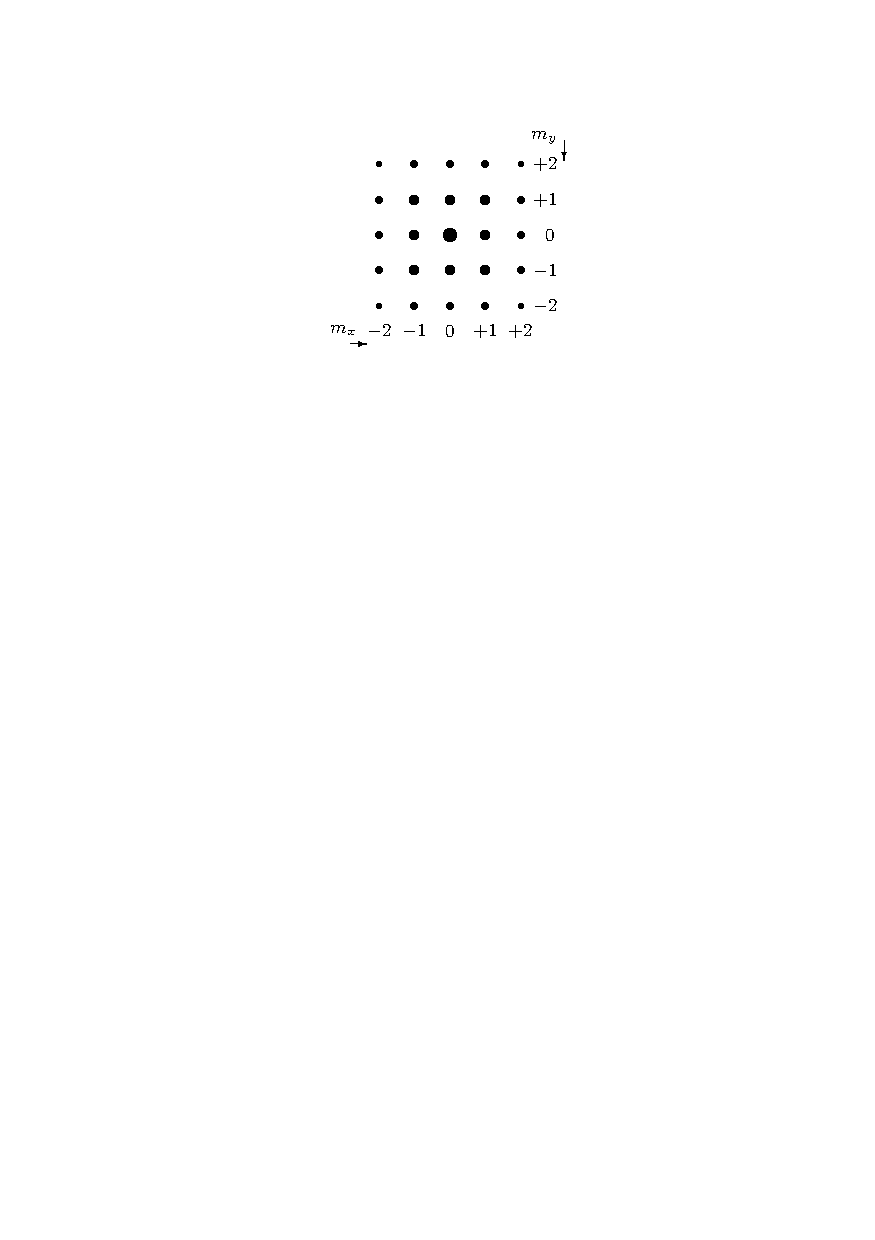
\includegraphics[scale=1.0]{max.pdf}}
		\caption{Дифракция Фраунгофера на двумерной решётке (сетке). Максимумы изображены кружками, размеры которых характеризуют интенсивности.}
		\label{ris:max}
	\end{figure}
	
	Если теперь поместить в фокальной плоскости щель так, чтобы через неё проходили дифракционные максимумы с $m_x = 0$ и $m_y =0, \pm 1, \pm 2, ...$ (с $m_y = 0$ и $m_x =0, \pm 1, \pm 2, ...$), то в плоскости $P_2$ получится изображение решётки с горизонтальными (вертикальными) штрихами. Таким образом можно продемонстрировать явление \textit{пространственной фильтрации} -- выделение различных структур в изображении.
	\newpage
\section*{Экспериментальная установка}
	Схема модели проекционного микроскопа приведена на рис.~\ref{ris:ustanovka}. Предметом служат сетки, расположенные в кассете. Смена сеток осуществляется поворотом внешнего кольца кассеты.
	\begin{figure}[H]
		\center{
\includegraphics[scale=1.0]{ustanovka.pdf}}
		\caption{Схема экспериментальной установки -- модель проекционного микроскопа.}
		\label{ris:ustanovka}
	\end{figure}
	Изображение сетки периодически повторяется -- \textit{репродуцируется} -- в пространстве между сеткой и первой линзой. Для выделения геометрического изображения среди множества репродуцированных изображений сетки на одну из сеток наложена тонкая проволока, то есть непереодический объект, изображение которого не репродуцируется.
	
\section*{Ход работы}
\subsection*{Определение периода решёток по их пространственному спектру}

С помощью лазера на экране, удалённом от него на расстояние $L = 123,5$ см, были получены дифракционные картины для различных сеток и измерены расстояния $l$ между соседними дифракционными максимумами.
Таким образом, были найдены периоды решёток: $d = m \lambda / \sin \theta$, где $\sin \theta \approx l/L$, $m = 1$, $\lambda = 532$ нм.

\begin{table}[H]
\begin{tabular}{|c|c|c|c|} \hline
Номер N & 1    & 2     & 3     \\ \hline
l, мм   & 66,00   & 26,44 & 13,31 \\ \hline
d, мкм  & 9,95 & 24,85 & 49,37 \\ \hline
\end{tabular}
\end{table}


\subsection*{Определение периода решёток по изображению, увеличенному с помощью модели микроскопа}
Была собрана установка согласно рис. 1 и измерены её размеры: $a_1 = 166$ мм, $b_1 = 250$ мм, $a_2 = 25$ мм,  $b_2 = 734$ мм. Параметры линз: $f_1 = 110$ мм, $f_2 = 25$ мм.
С помощью диафрагмы и микрометрического винта были определены периоды изображений сеток $l$,
после чего с помощью формулы $d = l/\Gamma$, где $\Gamma = \frac{b_1b_2}{a_1a_2} \approx 44,22$ -- увеличение оптической системы, были рассчитаны периоды решёток:

\begin{table}[H]
\begin{tabular}{|c|c|c|c|}
\hline
Номер N & 1     & 2     & 3     \\ \hline
l, мм   & 2,2   & 1,0   & 4,8   \\ \hline
d, мкм  & 24,88 & 11,31 & 54,28 \\ \hline
\end{tabular}
\end{table}


\subsection*{Определение периодов решёток по оценке разрешающей способности микроскопа}
Диафрагма с микрометрическим винтом была помещена в фокальную
плоскость F линзы Л$_1$. Для второй и третьей решётки был определён минимальный размер диафрагмы $D$, при котором на экране ещё видно изображение сетки. (Для первой определить не удалось из-за выхода за пределы диафрагмы). Из формулы (1) следует, что $d =~2\lambda f_1 / D$:


\begin{table}[H]
\begin{tabular}{|c|c|c|c|}
\hline
Номер N & 1  & 2        & 3    \\ \hline
D, мм   & -- & 5,36     & 1,9  \\ \hline
d, мкм  & -- & 21,83582 & 61,6 \\ \hline
\end{tabular}
\end{table}

\begin{figure}[H]
	\center{
\includegraphics[scale=0.5]{1.pdf}}
	\caption{График зависимости $d(1/D)$}
\end{figure}

Из графика видно, что аппроксимирующая прямая не проходит через 0, что связано с неточностью определения ширины диафрагмы и восприятия изображения на экране. Тем не менее, можно считать, что теория Аббе подтверждена.

\subsection*{Явление пространственной фильтрации}
Перед лазером была установлена сетка средних размеров (номер 2) с достаточно крупным вторичным изображением.
Ширина щели была подобрана так, чтобы она свободно пропускала
максимум нулевого порядка и не пропускала максимумы первого порядка, расположенные в поперечном направлении.
Поворачивая щель относительно оси системы, мы получили изображения решёток при различных
ориентациях щели: вертикальной, горизонтальной и наклонной под углом 45$^o$.

\begin{itemize}
    \item \textbf{Щель вертикальна:} Пропускается центральный максимум $(0,0)$ и все максимумы, лежащие на горизонтальной линии $(m_x = 0, \pm 1, \pm 2, \ldots, m_y = 0)$. В формировании изображения участвуют лучи только от вертикальных штрихов. Поэтому на экране видна вертикальная периодическая структура.
    \item \textbf{Щель горизонтальна:} Пропускается центральный максимум и все максимумы, лежащие на вертикальной линии $(m_x = 0, m_y = 0, \pm 1, \pm 2, \ldots )$. В изображении участвуют лучи только от горизонтальных штрихов. Поэтому на экране видна горизонтальная периодическая структура.
    \item \textbf{Щель под углом $45^\circ$:} Щель поставлена так, что она пропускает центральный максимум и те максимумы, которые лежат на линии, повернутой на $45^\circ$. Это те максимумы, у которых $m_x = m_y$, то есть $(1,1)$, $(-1,-1)$, $(2,2)$, $(-2,-2)$ и т.д.
        % Максимум $(1,1)$ образуется в результате дифракции на структуре, которая является диагональной составляющей твоей решётки.
        Когда интерферируют волны, идущие от центрального максимума $(0,0)$ и от максимумов типа $(1,1)$ и $(-1,-1)$, они создают интерференционную картину, период которой направлен перпендикулярно линии, соединяющей эти максимумы.
Так как максимумы $(1,1)$ и $(-1,-1)$ лежат на линии под $45^\circ$, то интерференционные полосы будут ориентированы под углом $90^\circ$ к этой линии, то есть тоже под $45^\circ$, но в другую сторону. В результате получается изображение периодической структуры, ориентированной под углом $45^\circ$.
\end{itemize}
\begin{figure}[H]
	\center{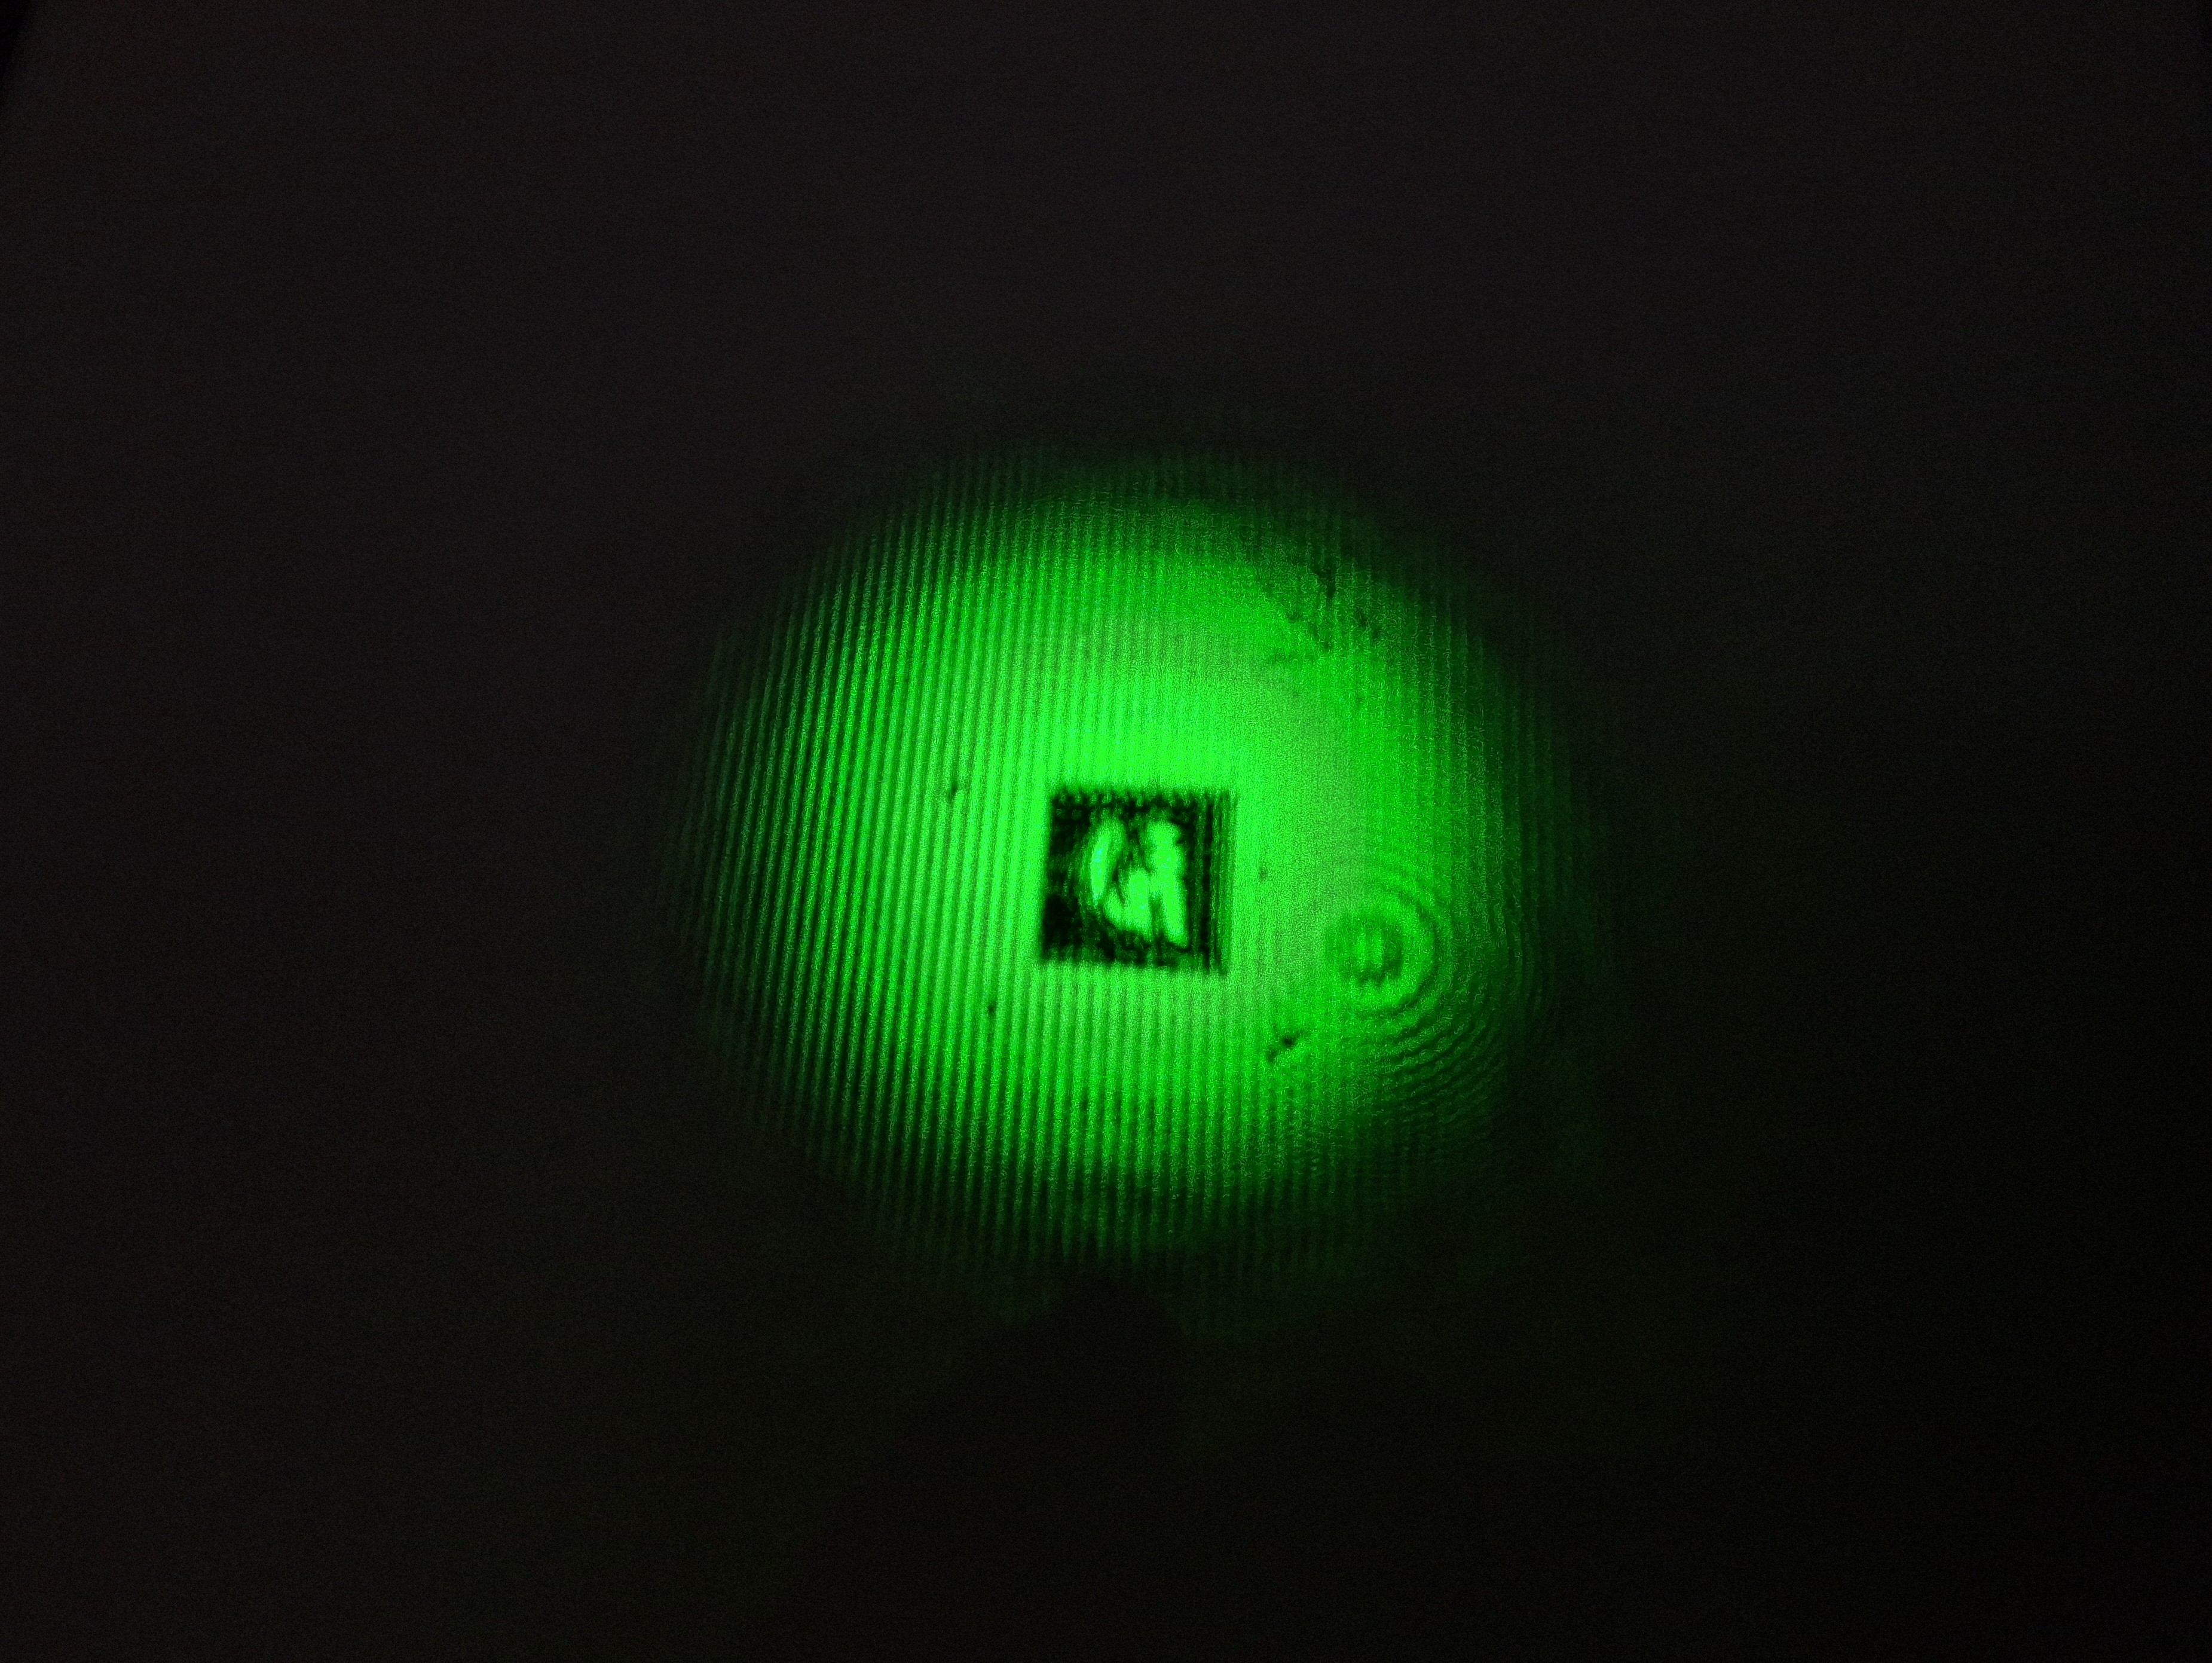
\includegraphics[scale=0.11]{20260226_105318.jpg}}
	\caption{Вертикальное положение}
\end{figure}

\begin{figure}[H]
	\center{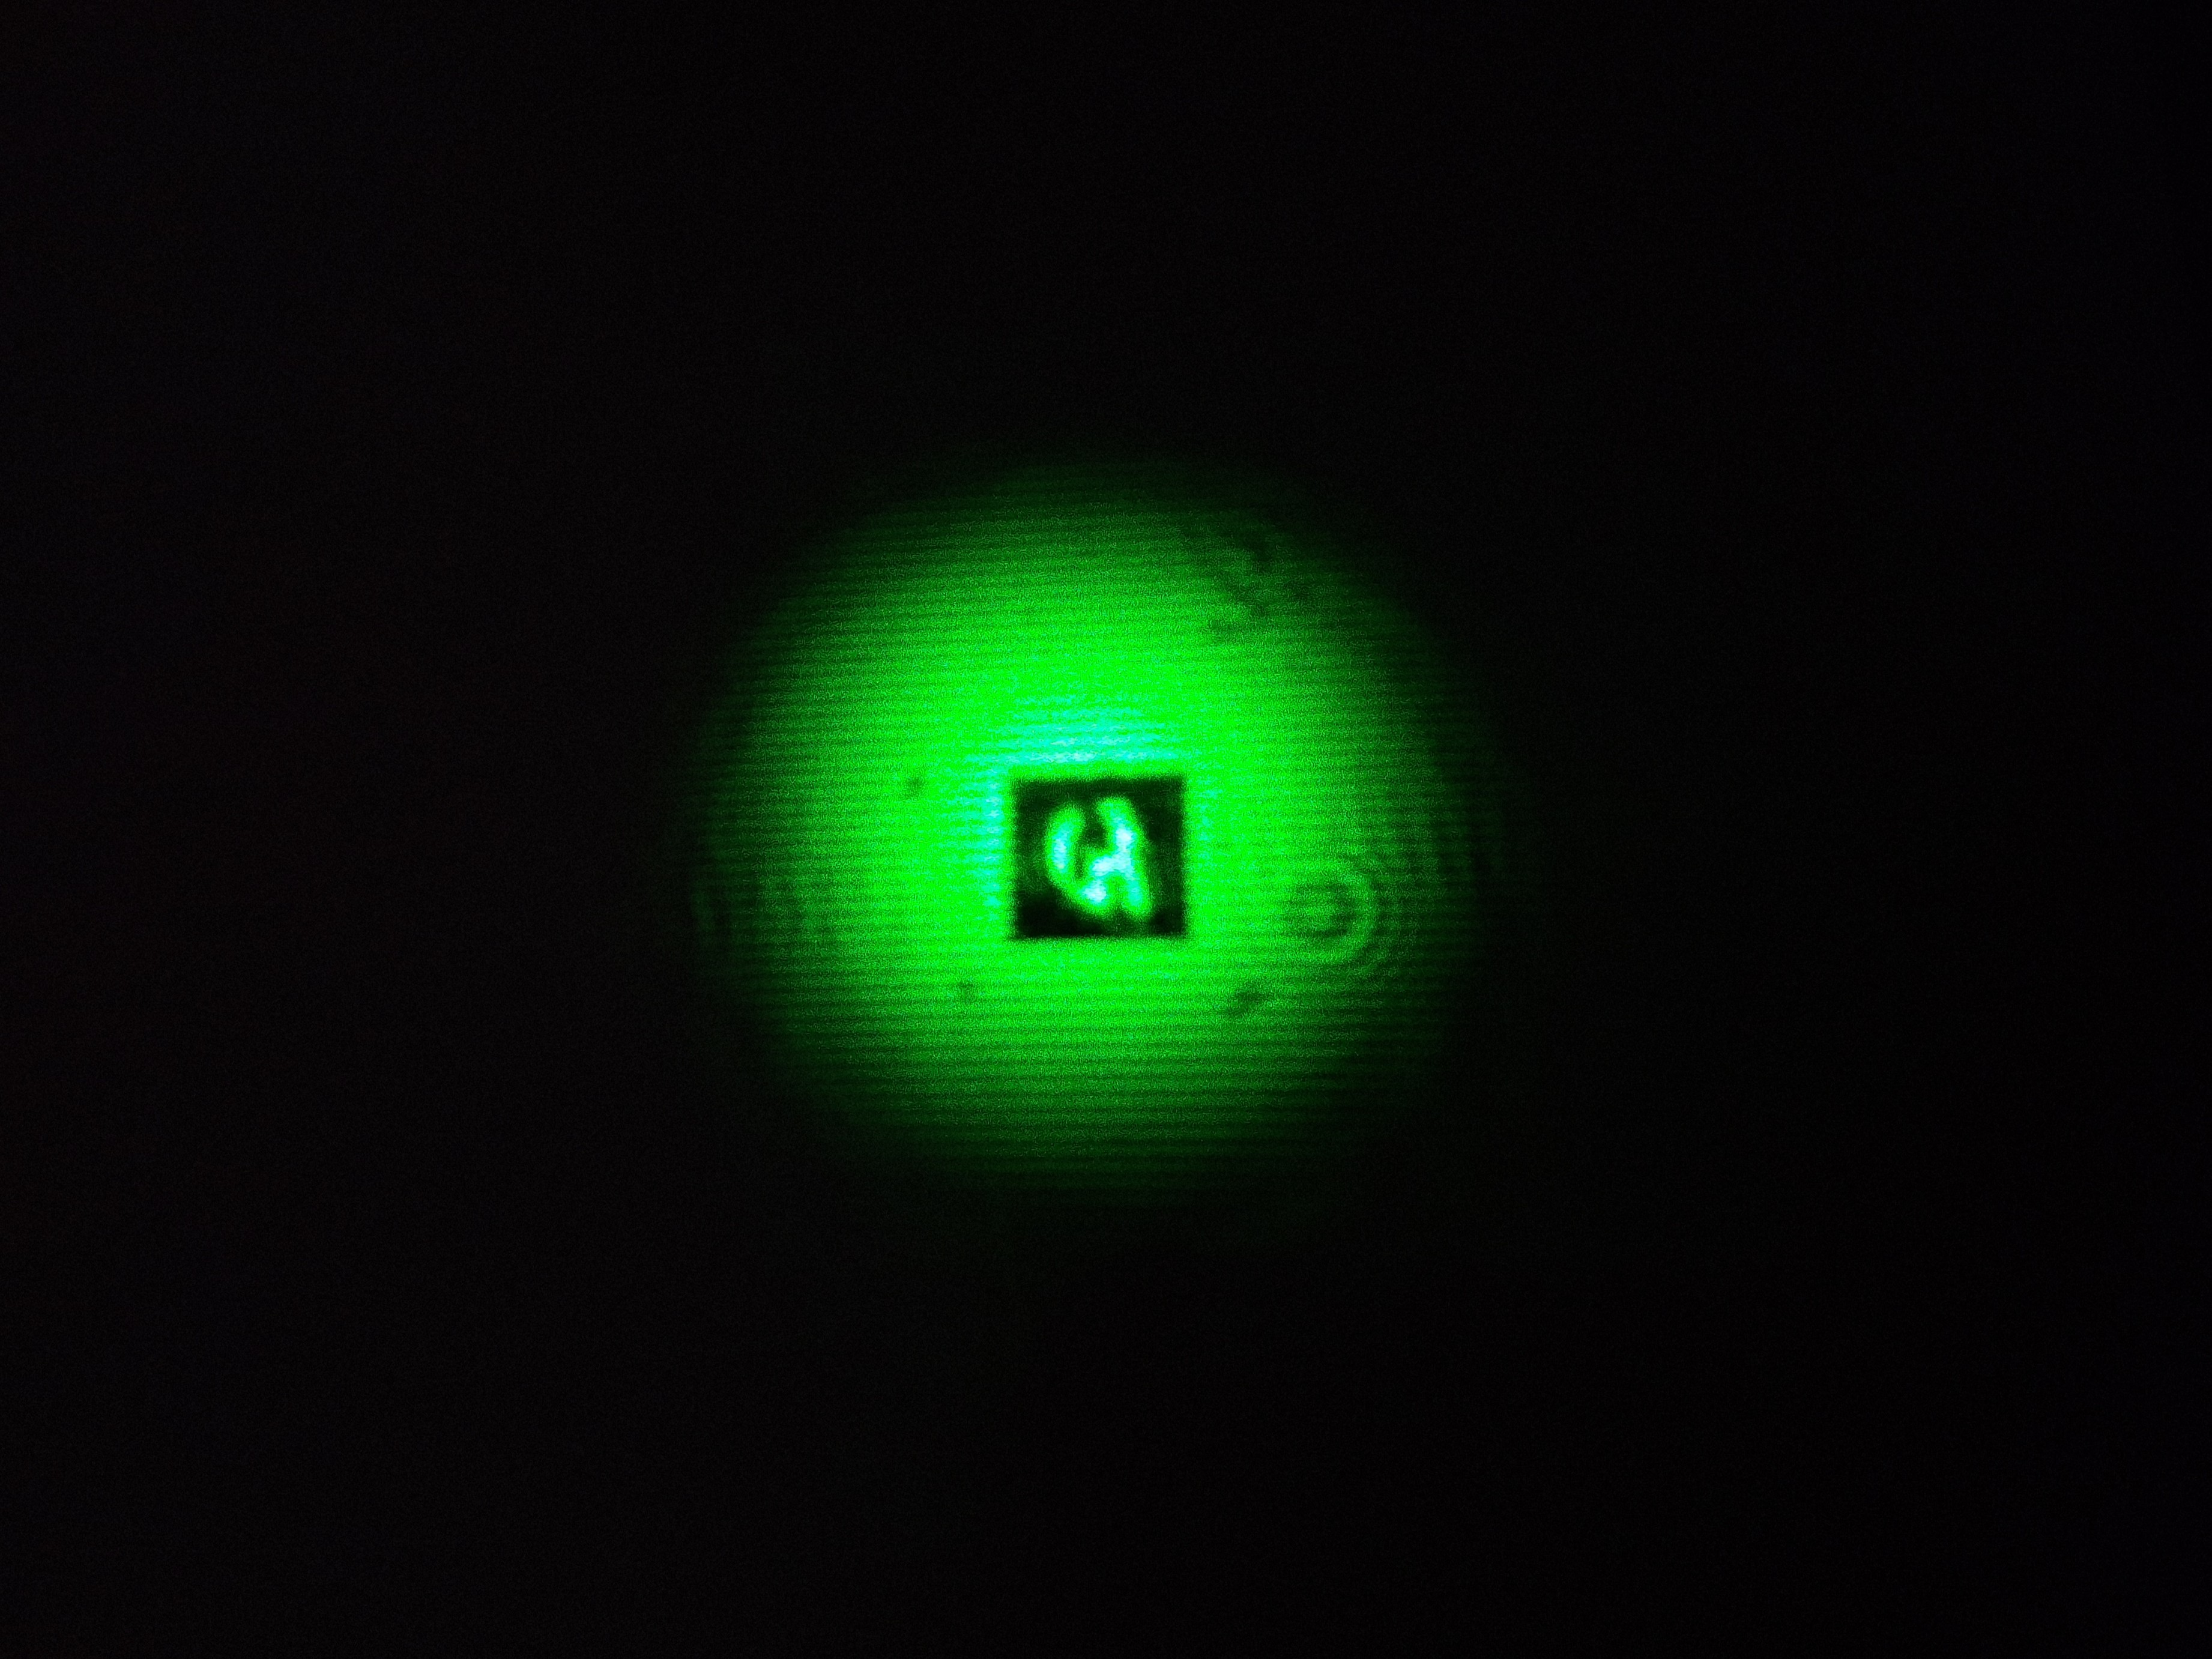
\includegraphics[scale=0.11]{20260226_105106.jpg}}
	\caption{горизонтальное положение}
\end{figure}

\begin{figure}[H]
	\center{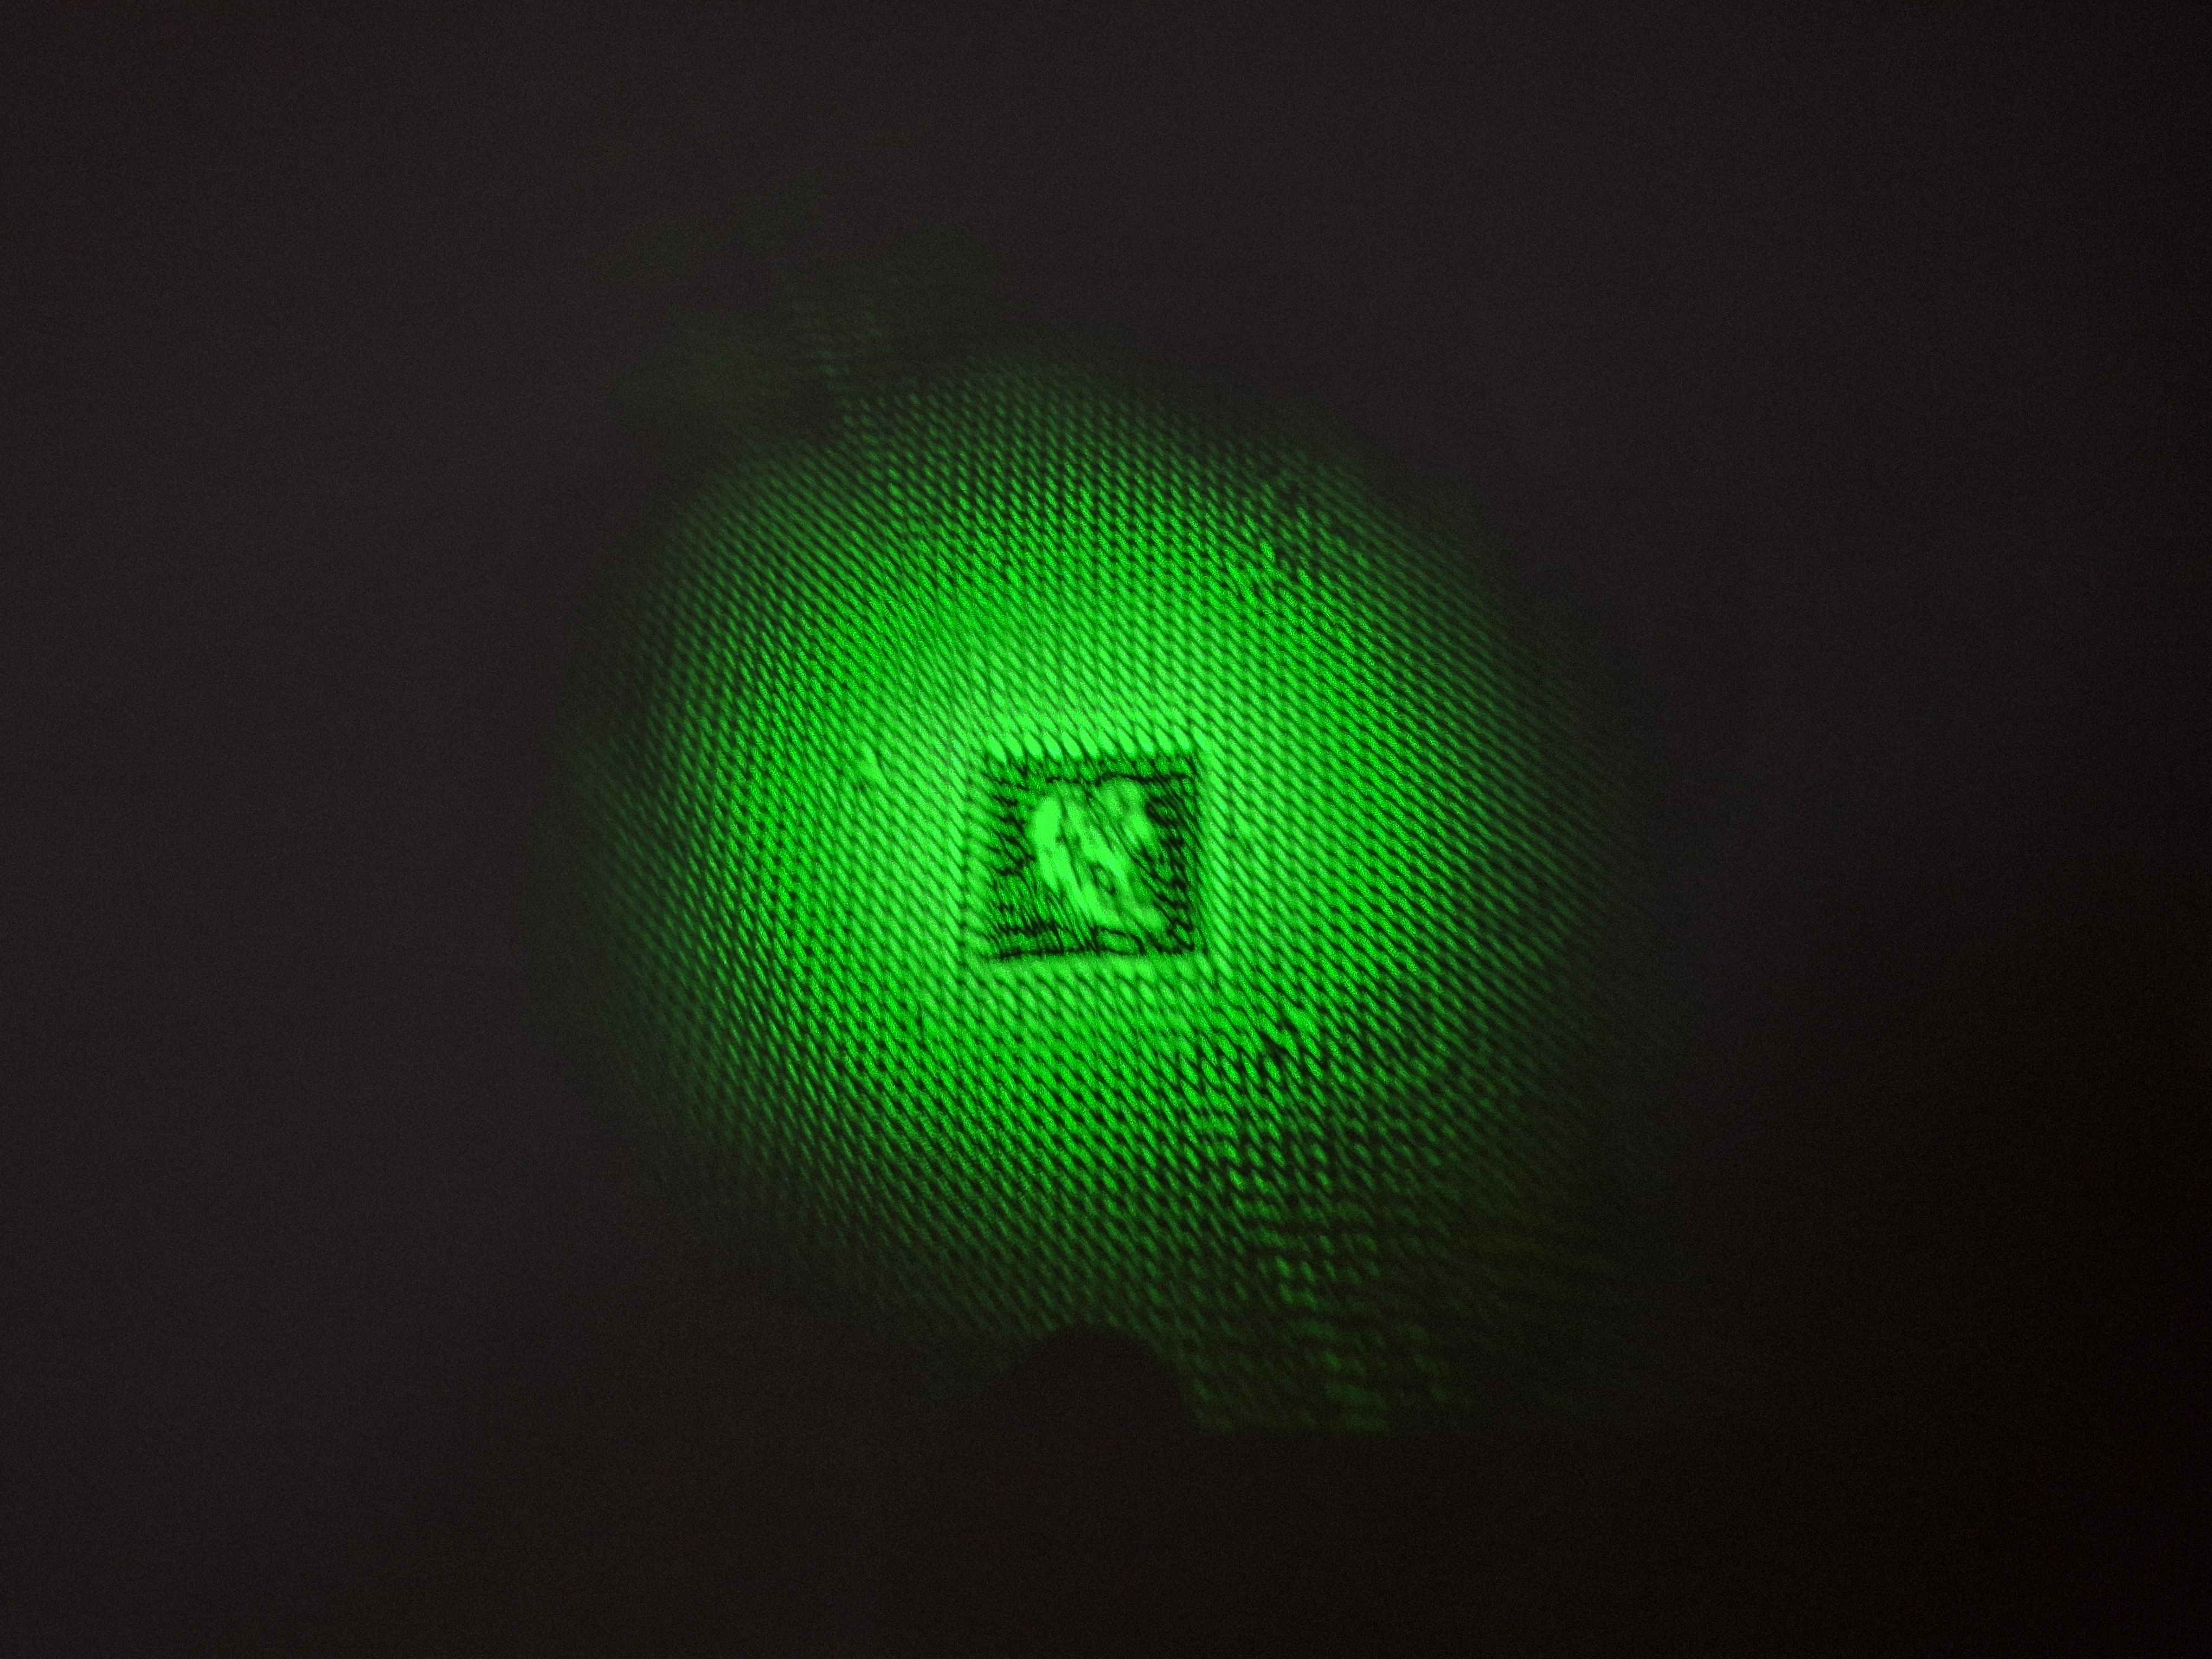
\includegraphics[scale=0.1]{20260226_105528.jpg}}
	\caption{Наклонное положение}
\end{figure}


\subsection*{Явление мультиплицирования}
Для наблюдения явления мультиплицирования были поменяны местами сетка и щель: сначала было получено резкое
изображение щели, а затем в фокальной плоскости F объектива поставлена
кассета с сетками, которые рассекали фурье-образ щели.
Была подобрана такая ширина входной щели D, чтобы на экране можно
было наблюдать мультиплицированное изображение для всех сеток.

При сужении ширины щели на экране было заметно лишь сужение каждого мультиплицированного изображения,
а при смене сетки на более крупную появилось больше копий изображения.
Это вызвано тем, что дифракционные максимумы (отверстия в фурье-плоскости) крупной сетки расположены более часто, и через них проходит больше порядков спектра щели, создавая на экране больше копий изображения.

\begin{figure}[H]
	\center{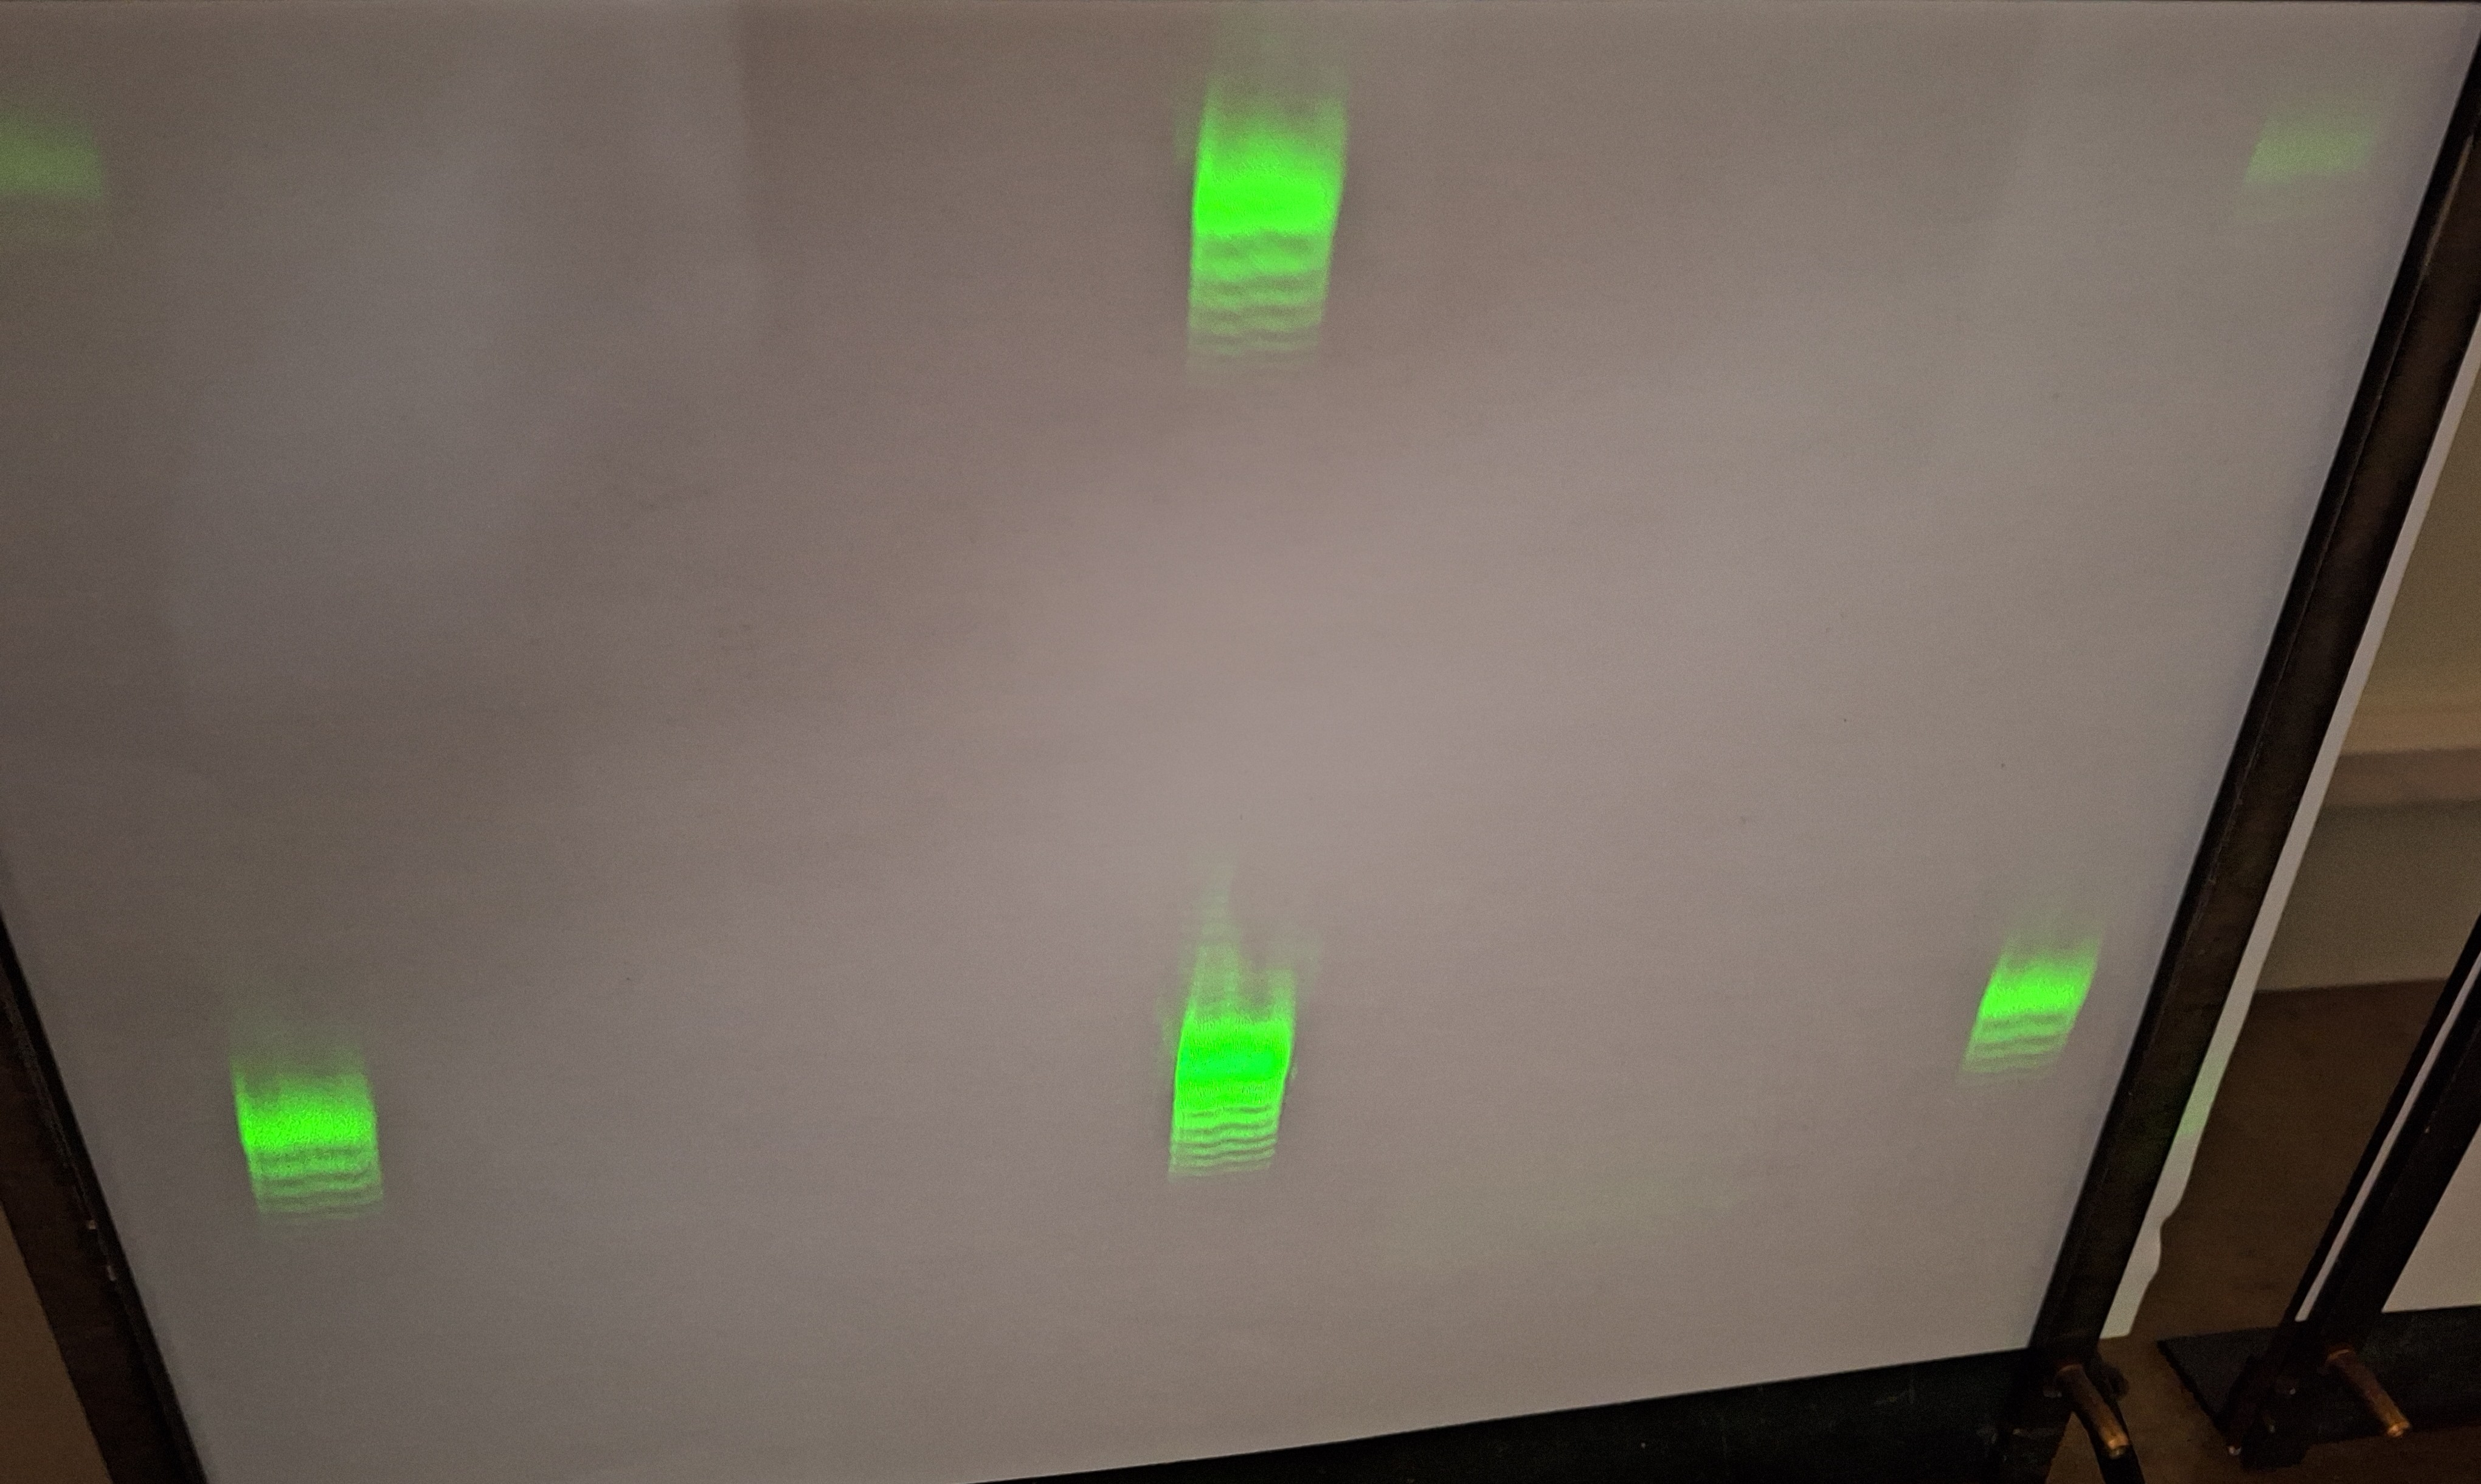
\includegraphics[scale=0.1]{20260226_110110.jpg}}
	\caption{Решётка номер 2}
\end{figure}

\begin{figure}[H]
	\center{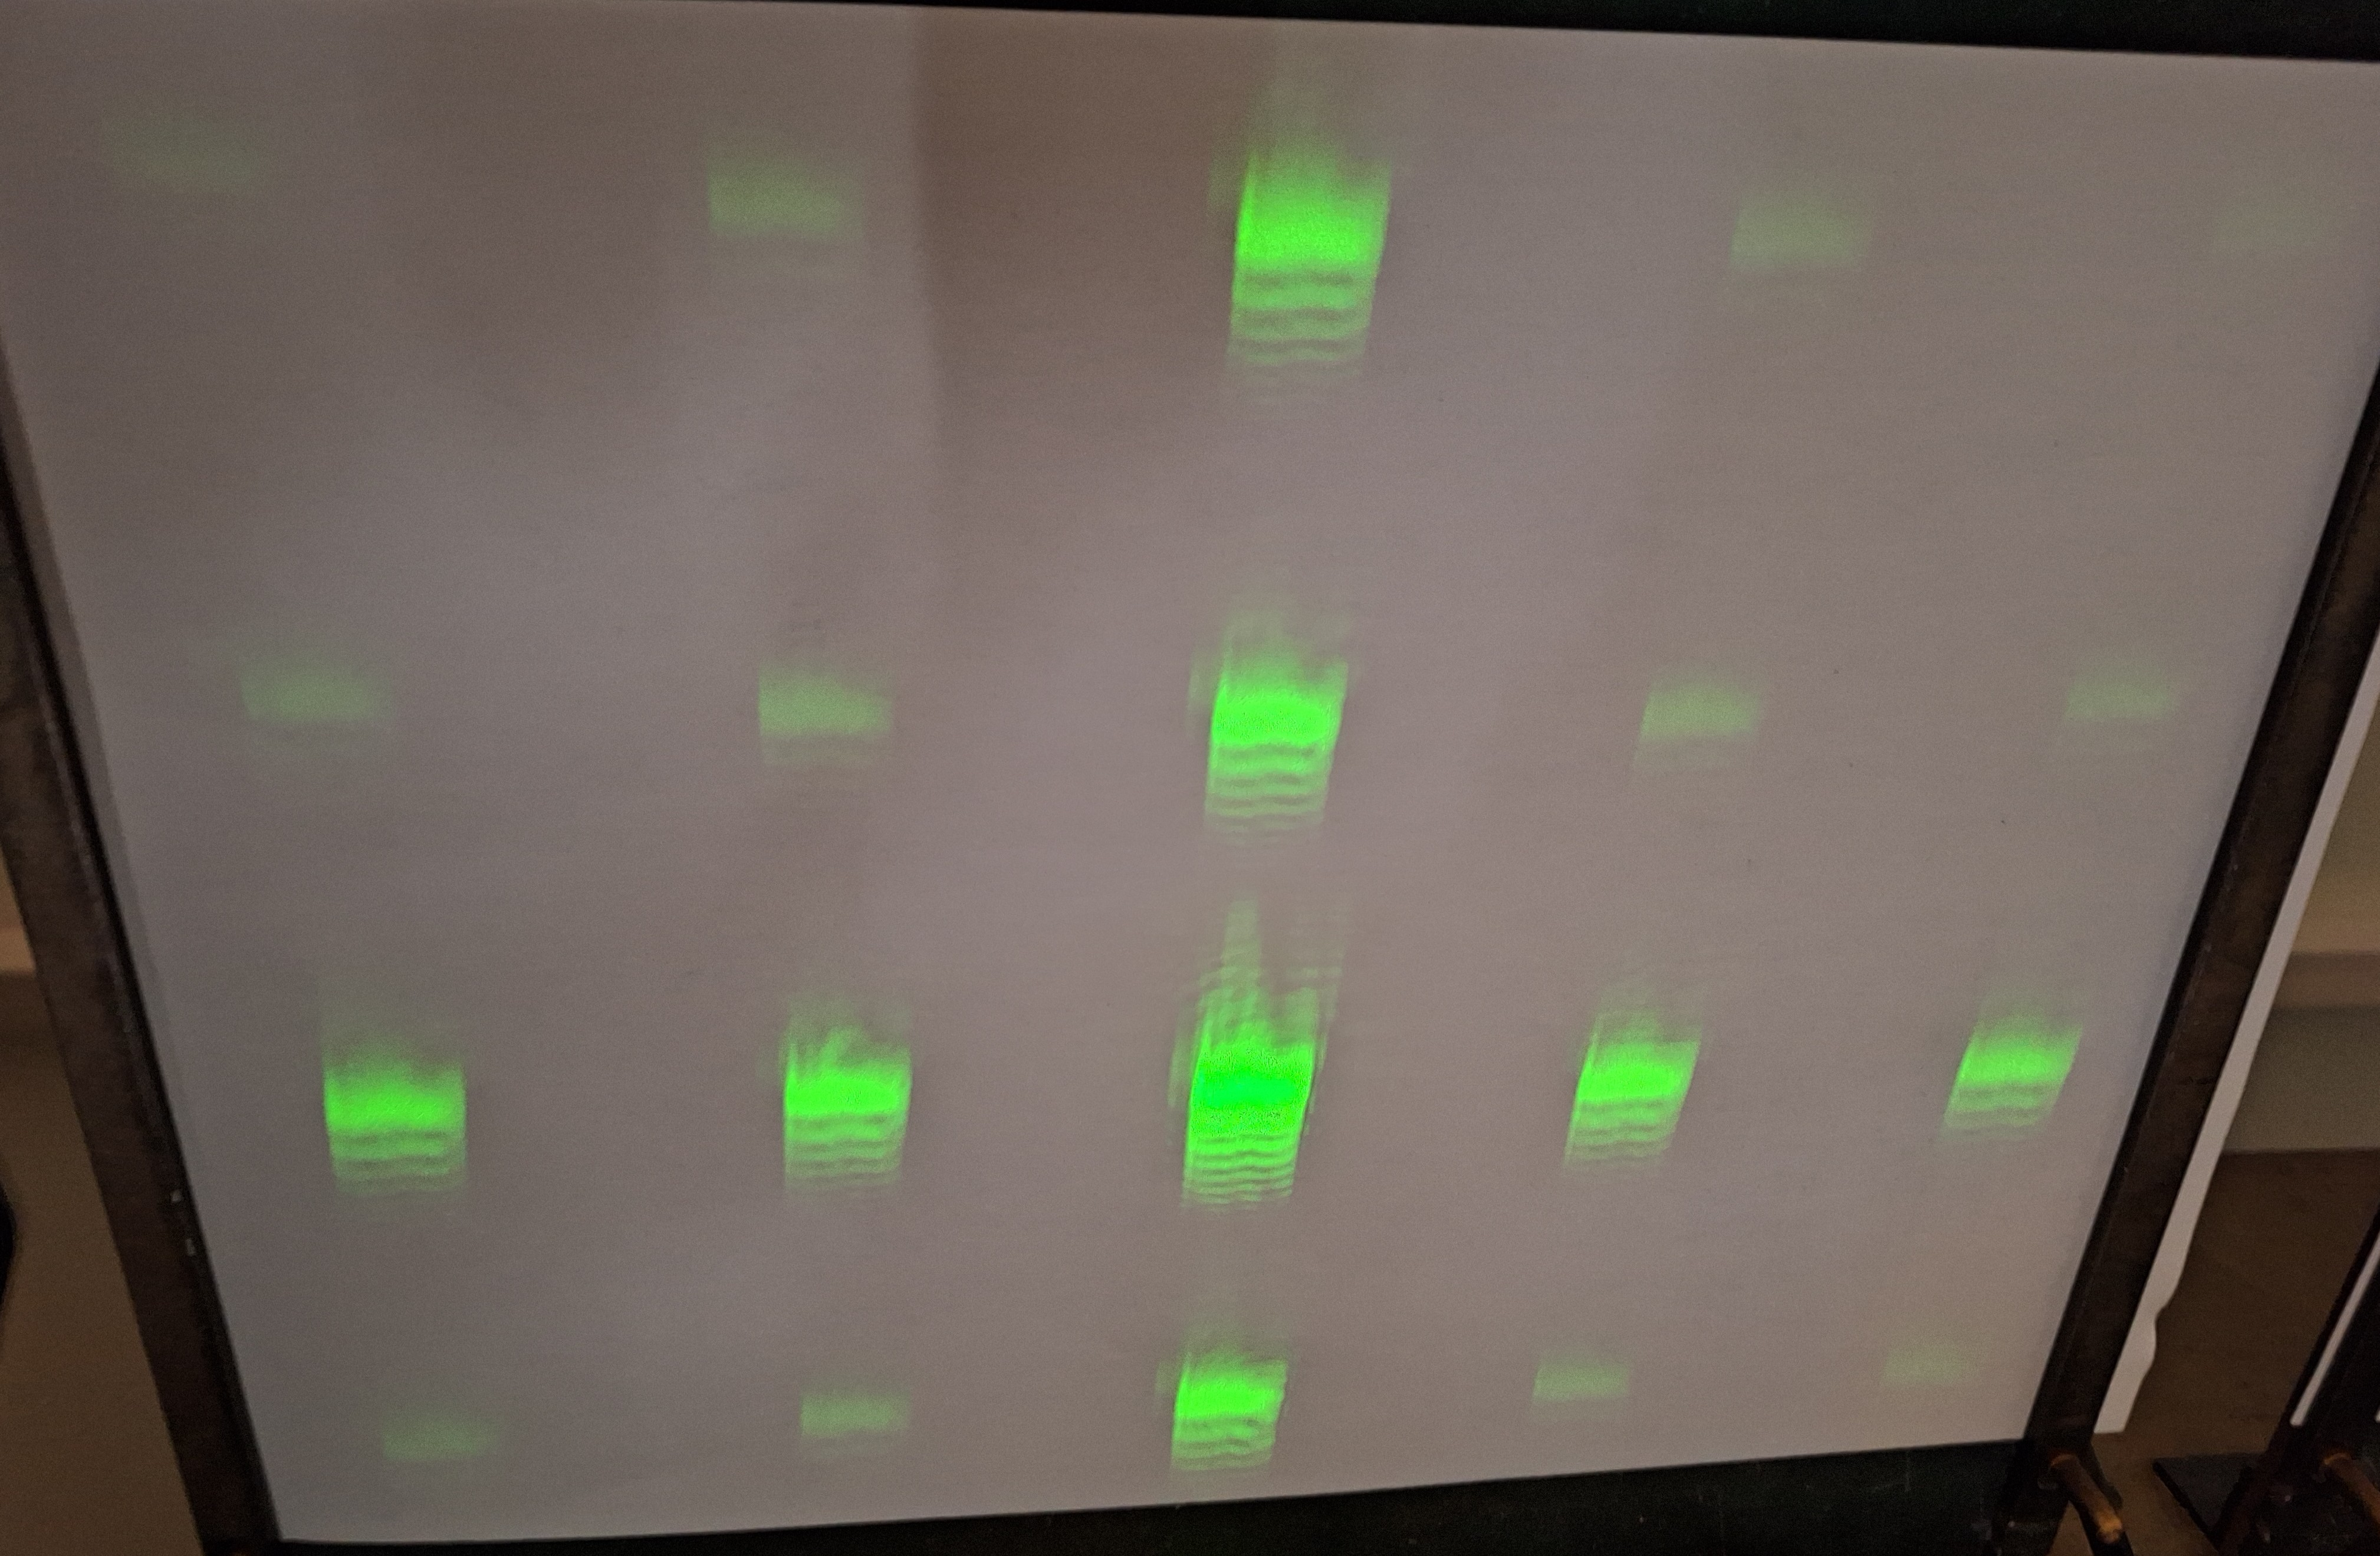
\includegraphics[scale=0.1]{20260226_110304.jpg}}
	\caption{Решётка номер 3}
\end{figure}



\section*{Выводы}
\begin{table}[H]
\centering
% \caption{Сводная таблица результатов определения периодов сеток}
\begin{tabular}{|c|c|c|c|}
\hline
$N$ & $d$, мкм (спектральный метод) & $d$, мкм (увеличение) & $d$, мкм (разрешающая способность) \\
\hline
1 & 9,95 & 24,88 & --- \\ \hline
2 & 24,85 & 11,31 & 21,84 \\ \hline
3 & 49,37 & 54,28 & 61,60 \\
\hline
\end{tabular}
\end{table}

В ходе работы была экспериментально проверена теория Аббе о дифракционном пределе разрешения микроскопа. Периоды сеток, измеренные тремя независимыми методами, получились приблизительно одинаковыми. Наблюдаемые расхождения связаны с неточностью определения положения линз, измерений на экране и субъективностью критерия видимости изображения. Качественные опыты по пространственной фильтрации и мультиплицированию наглядно подтвердили, что изображение формируется в результате интерференции дифракционных максимумов, и, изменяя их набор в фокальной плоскости, можно управлять структурой изображения.


\end{document}